% !Mode:: "TeX:UTF-8"

\chapter{系统整体设计}[overall]
\label{chapter:overall}

本章简明描述本文所设计的操作系统的体系结构和主要的构成模块,旨在对整个操作系统有一个整体的把握。当前暂时将这个操作系统命名为“Moonix”,后文中的“Moonix”皆指本文所设计实现的操作系统。

目前,整个Moonix操作系统设计有两个部分组成:监管者模式部分和用户模式部分。监管者模式部分即操作系统内核,用于对硬件资源进行抽象和调度访问,向下沟通位于机器模式的SBI,向上应答用户模式的服务请求。用户模式部分,即操作系统服务,目前主要实现的是内核编程接口,用户编写的程序不会直接向监管者模式请求服务,而是通过调用内核编程接口函数,由这些函数代为请求。

Moonix整体采用了宏内核模式。宏内核的优点是执行速度快,缺点则是层次结构性不强。尽管如此,我们还是可以将其大概划分为以下四个模块:中断处理模块、内存管理模块、进程调度模块和文件系统模块。从宏内核模式结构模型(分层思想)出发,我们可以将Moonix的层次结构大致描述为图 \ref{pic:moonixtotal}。

\begin{figure}[htpb]
	\centering
	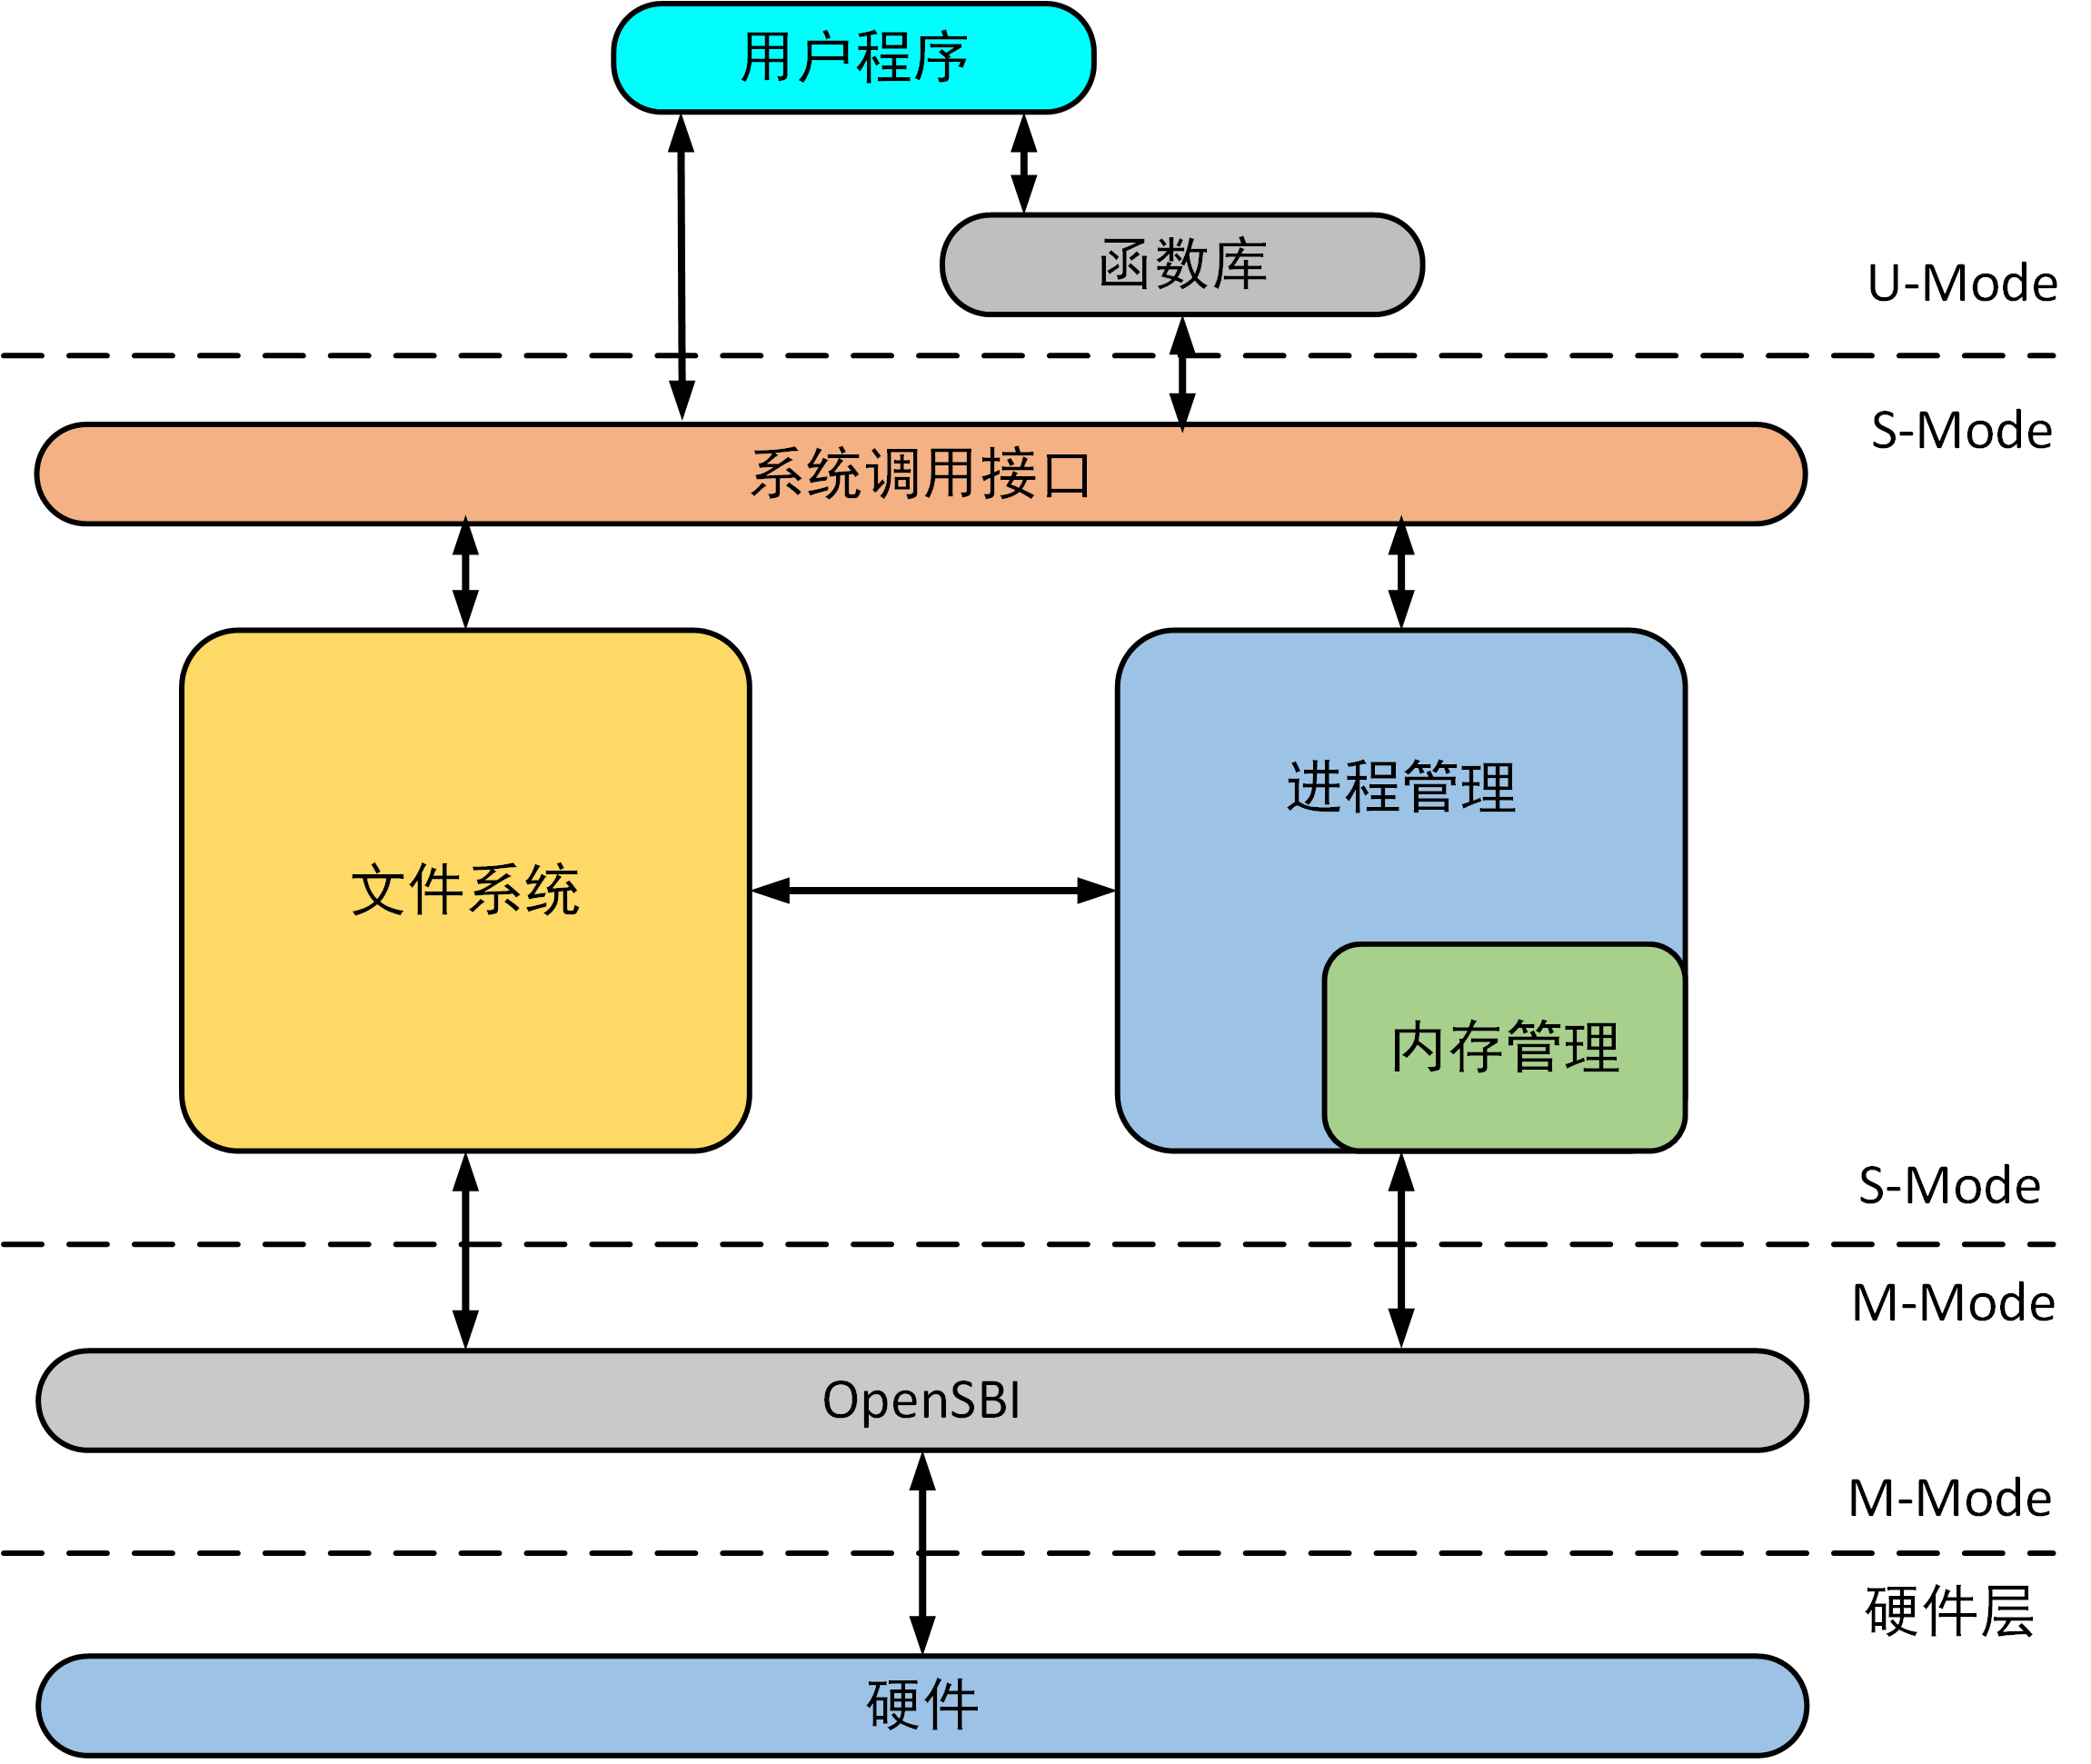
\includegraphics[width=0.75\textwidth]{moonixtotal.png}
	\setlength{\abovecaptionskip}{2pt}
	\caption{Moonix体系结构}
	\label{pic:moonixtotal}
\end{figure}

中断处理模块用于控制操作系统对内外部中断的响应。操作系统通过响应定时器中断,来定时检查进程的运行状态,可以说中断处理是进程调度的基础。内存管理模块主要通过虚拟内存管理的方式,保证各个进程能够安全共享物理内存,互不干扰。同时,由于各个进程都运行在独立的虚拟内存空间,实现程序时不必考虑实际的物理内存状态,降低了应用程序的实现难度。进程调度模块用来控制一个进程是否可以占用CPU运行,通过Round-Robin算法\cite{DBLP:journals/eor/RasmussenT08},来保证各个进程都有相同的机会来执行代码。文件系统模块提供了一个通用的文件接口,操作系统可以不用关心不同类型文件的具体实现,而进行统一的文件读写操作。

Moonix操作系统目前只能运行在QEMU虚拟机模拟的virt计算机上\cite{qemu/virt},以OpenSBI作为SBI。因此,Moonix可管理的内存受制于virt和OpenSBI。整个virt计算机可用物理内存大小为128MB,除去OpenSBI和Moonix内核占据的内存外,其余的内存都是Moonix操作系统可以管理的内存区域。

Moonix采用RISC-V指令集架构提供的Sv39系统来对内存进行虚拟化管理。Moonix将全部的128MB物理内存映射到一个512GB大小的虚拟地址空间中,并通过填充页表来对这种映射关系进行管理,CPU在进行地址解析时就可以通过页表来执行自动的地址翻译。在Moonix中,不同的进程可以拥有不同的页表,这意味着它们运行在相互隔离的虚拟地址空间中。当一个用户进程在运行时,虚拟地址空间和虚拟地址空间的布局和映射关系如图 \ref{pic:moonixmem} 所示。

\begin{figure}[htpb]
	\centering
	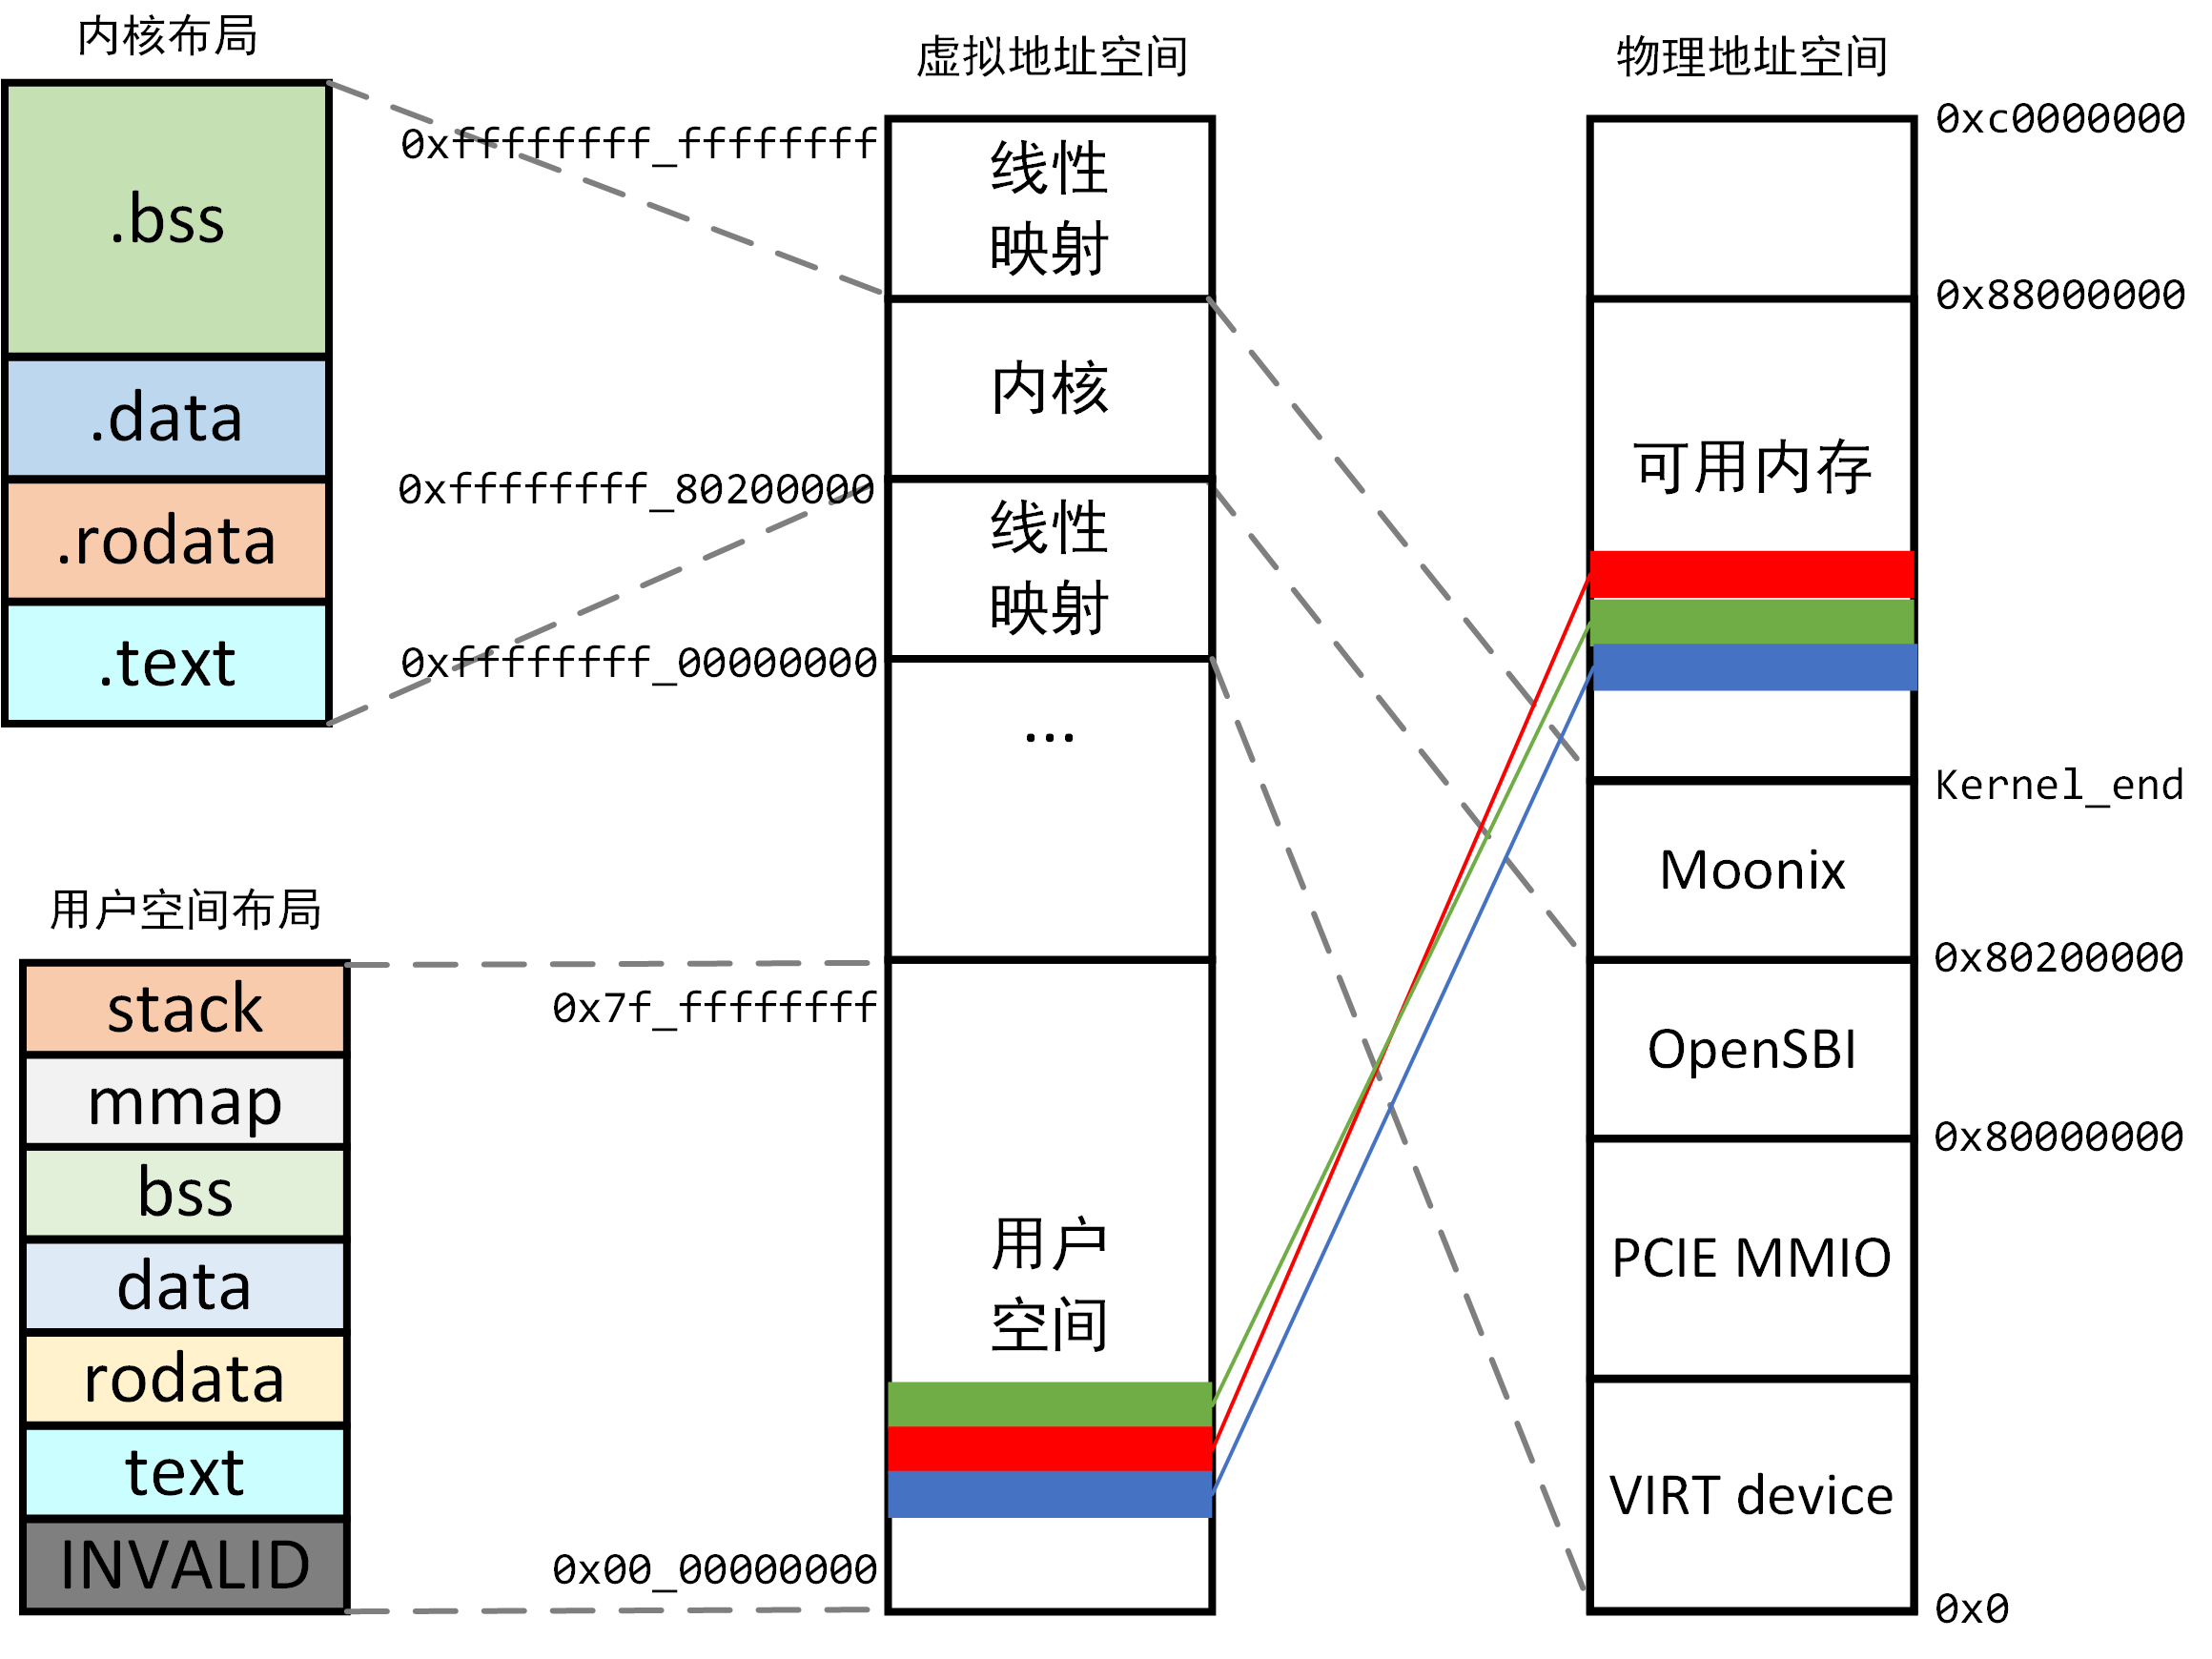
\includegraphics[width=0.85\textwidth]{mem.png}
	\setlength{\abovecaptionskip}{2pt}
	\caption{Moonix内存结构}
	\label{pic:moonixmem}
\end{figure}

在进程的虚拟地址空间中,进程的私有代码和数据占据了低地址空间,而内核的代码和数据占据了高地址空间。内核需要被映射到每个进程的高地址处,来保证用户进程在发起系统调用陷入内核时,进程能够寻找到内核的处理代码。

\begin{figure}[htpb]
	\centering
	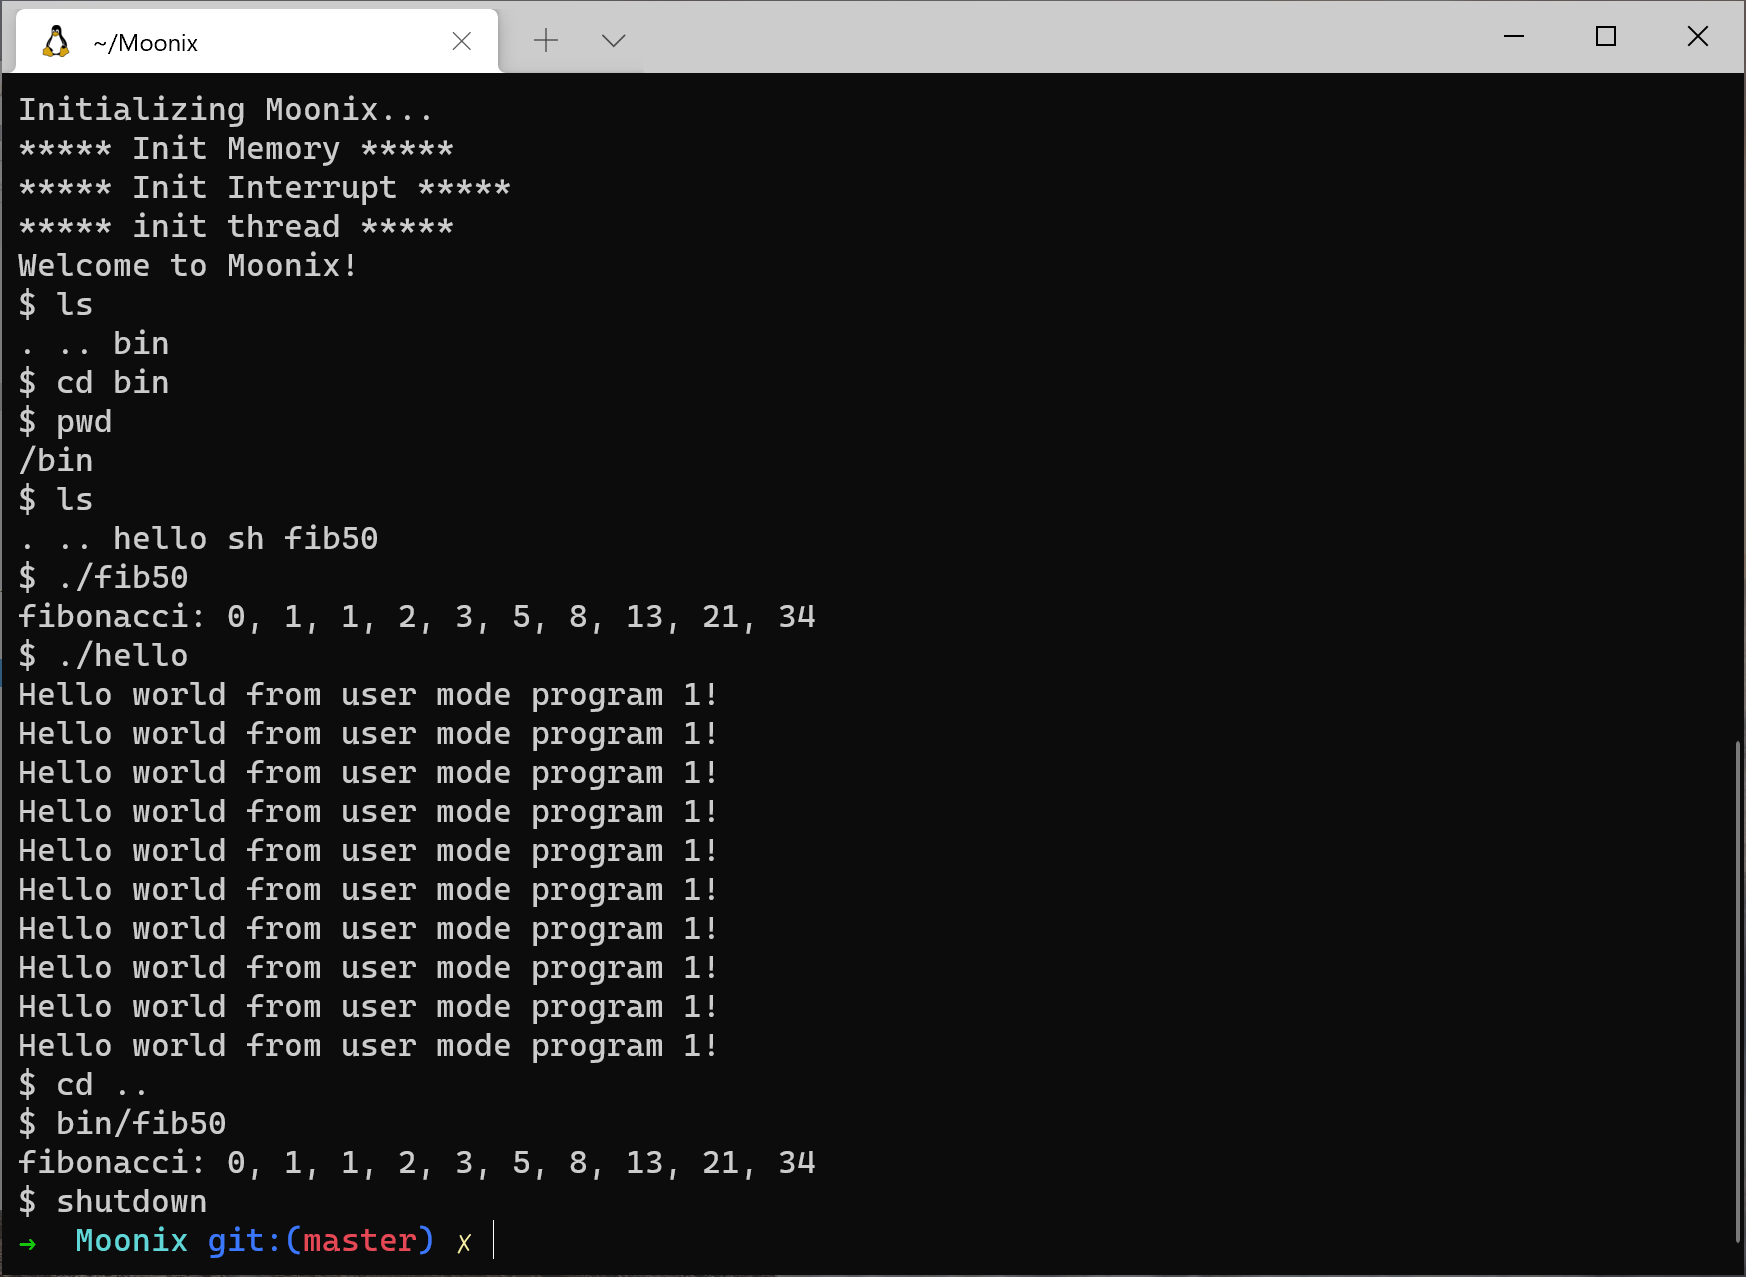
\includegraphics[width=\textwidth]{MoonixRun.png}
	%\setlength{\abovecaptionskip}{2pt}
	\caption{Moonix运行效果}
	\label{pic:moonixrun}
\end{figure}

目前Moonix内置了两个简单的用户程序,分别是输出10遍相同字符串的hello程序,和计算并输出小于50的斐波那契数列的fib50,它们都位于文件系统上的 /bin文件夹中。

图 \ref{pic:moonixrun} 是当前Moonix操作系统的运行示例。在Moonix初始化结束之后,会输出“Welcome to Moonix!”,并启动一个可交互的shell进程。用户可以在shell中输出简单的内置命令交互,或者输入可执行文件的路径来执行程序。shell目前内置cd、ls、pwd和shutdown命令。在示例中,用户首先cd到 /bin文件夹下,运行了fib50和hello程序,接着再cd回上一级文件夹,使用相对路径的方式再次执行了一次fib50程序,最后通过shutdown命令关闭Moonix系统。